\section{Manual del Usuario. Tamtam Listens}

\subsection{¿Qu\'e es TamTam?}

TamTam es un compendio de cuatro actividades relacionadas con la m\'usica y sonido para la XO.
TamTam Edit es una de \'estas actividades y proporciona una interfaz para crear, modificar y organizar
notas ubicadas en cinco ``pistas'' virtuales. Adem\'as incluye una paleta de casi cien tipos de sonidos y
modelos de construcci\'on musical que permite crear distintos tipos de variaciones en estilos musicales.
Las secciones principales del programa se pueden observar en la siguiente figura:


\begin{figure}[H] 
\centering
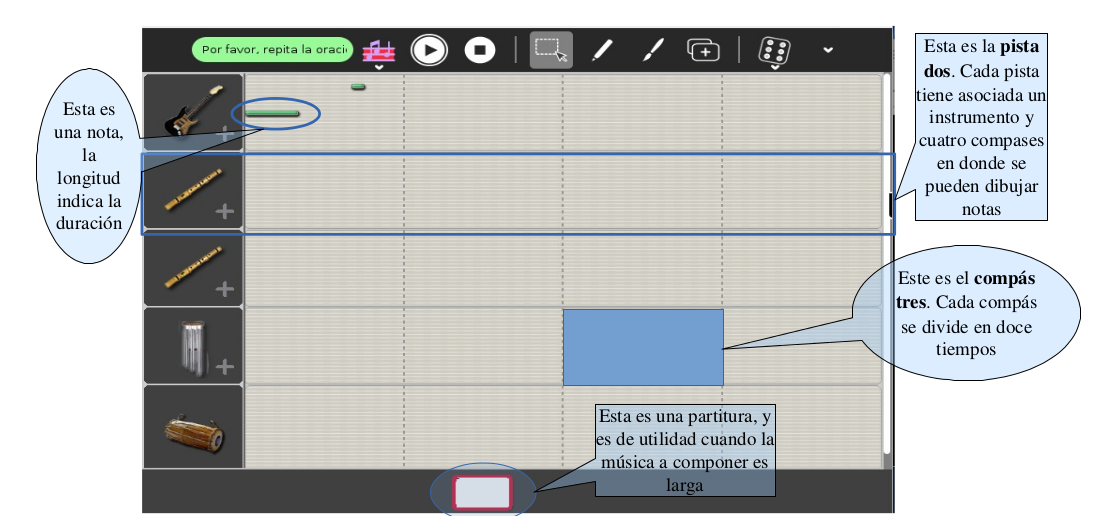
\includegraphics[width=1\textwidth]{./graphics/ui-tamtam.png}
\caption{Interfaz de TamTam Edit y sus secciones principales}
\label{figure:ui-tamtam-anexo}
\end{figure}

Como se puede apreciar la interfaz se encuentra organizada en cinco pistas y cada pista tiene asociada
un instrumento (la quinta pista esta reservada para instrumento de tipo bater\'ia). Cada pista se divide en
4 compases (del comp\'as uno al cuatro) y cada comp\'as se divide en 12 tiempos (del uno al doce). Las
notas se dibujan en los compases, como se puede ver, la longitud de la nota indica su duraci\'on y su
altura el tipo de nota.  Adem\'as la aplicaci\'on esta organizada en partituras, que son como hojas  de
cuaderno, y son \'utiles para componer m\'usicas largas.

\subsection{TamTam Listens}
\foreign{Tamtam Listens} es una interfaz alternativa para la aplicaci\'on TamTam Edit, en la cual se puede
componer m\'usica utilizando comandos de voz. 

\subsubsection{¿C\'omo interactuar con la interfaz?}
Para que la aplicaci\'on pueda reconocer los comandos de voz sin mayores inconvenientes, los mismos
deben ser dichos de manera clara y sin pausas largas entre palabras. Adem\'as en la Figura 1 se puede
observar una caja de texto que sirve para notificar al usuario el estado del reconocedor. El color verde
indica que se acaba de procesar el comando  de voz   y,  en caso de  \'exito, se muestra el comando
reconocido, en caso contrario, se muestra un mensaje pidiendo repetir el comando.  Adem\'as, el color
verde indica que la aplicaci\'on esta lista para reconocer otro comando. Por otro lado, el color rojo indica
que se esta procesando el comando actual y la aplicaci\'on no esta disponible para nuevos comandos.
A continuaci\'on se muestran los comandos disponibles en \foreign{TamTam Listens}.

\subsection{Comandos Generales}

\begin{figure}[H] 
\centering
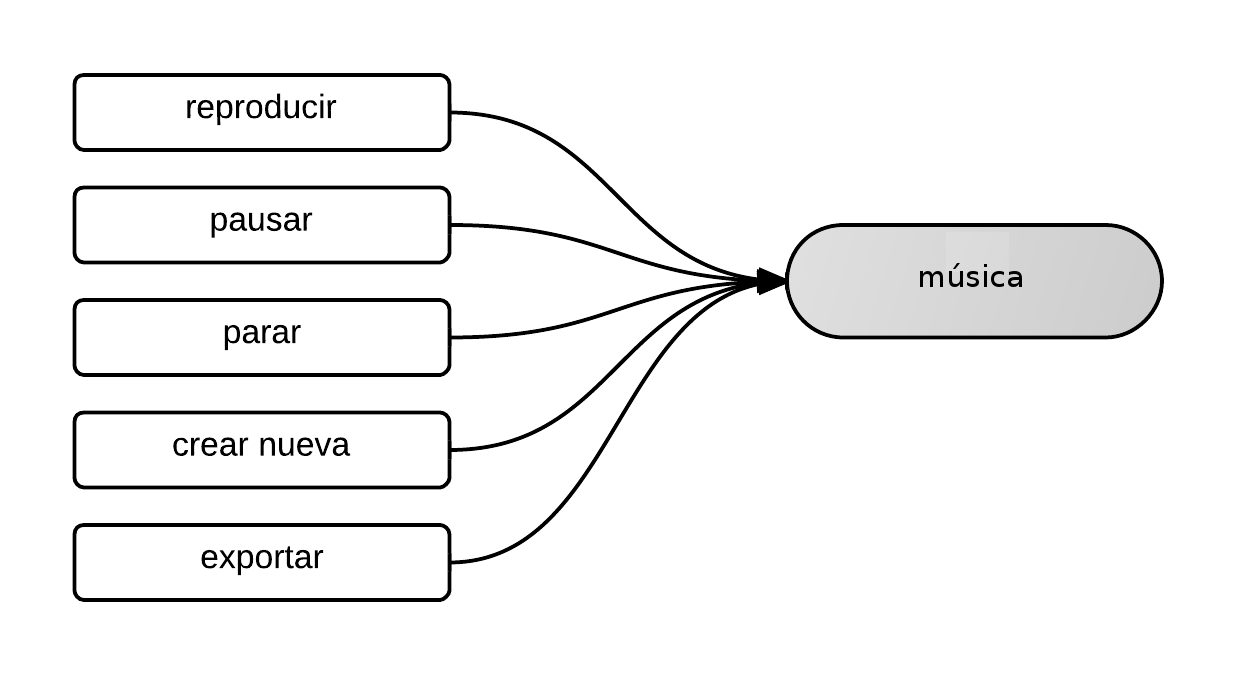
\includegraphics[width=0.5\textwidth]{./graphics/cmd-musica.png}
\caption{Comandos para reproducir, pausar, parar, exportar y crear una m\'usica}
\label{figure:cmd-crear-musica-anexo}
\end{figure}

\begin{itemize}
\item \emph{reproducir m\'usica}: permite reproducir la m\'usica creada.
\item \ emph{pausar m\'usica}: permite pausar la reproducci\'on actual dejando la l{\'\i}nea de reproducci\'on en el
punto de pausa.
\item \emph{parar m\'usica}: permite parar la reproducci\'on actual y ubica la l{\'\i}nea de reproducci\'on al inicio de
la m\'usica.
\item \emph{crear nueva m\'usica}:  permite crear una nueva composici\'on, dejando como resultado una
partitura en blanco.
\item \emph{exportar m\'usica}: permite guardar la m\'usica creada en un archivo para que reproducirse en un
reproductor multimedia.
\end{itemize}

Cabe destacar que cuando se esta reproduciendo una m\'usica, la aplicaci\'on solo acepta los comandos de
voz pausar m\'usica o parar m\'usica.


\begin{figure}[H]
\begin{minipage}[b]{0.5\linewidth}
\centering
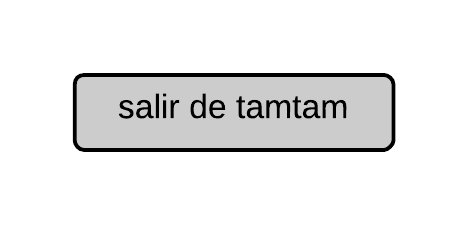
\includegraphics[width=0.6\linewidth]{./graphics/salir.png}
\caption{Comando para salir de la aplicaci\'on}
\label{figure:cmd-salir-anexo}
\end{minipage}
\quad
\begin{minipage}[b]{0.5\linewidth}
\centering
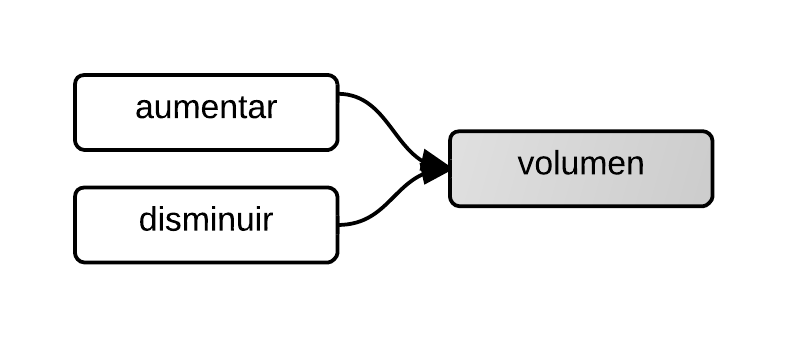
\includegraphics[width=0.6\linewidth]{./graphics/cmd-vol.png}
\caption{Comandos para aumentar/disminuir el volumen general}
\label{figure:cmd-vol-anexo}
\end{minipage}
\end{figure}

El comando de la figura~\ref{figure:cmd-salir-anexo} permite salir de \emph{TamTam Listens}, simplemente hay que decir ``salir de tamtam''. Por otro lado, los comandos de la figura~\ref{figure:cmd-vol-anexo}
y~\ref{figure:cmd-tempo} permiten controlar, respectivamente, el volumen y tempo general de la aplicaci\'on. Por ejemplo: ``aumentar volumen'', ``disminuir tempo''.

 \begin{figure}[H]
\begin{minipage}[b]{0.5\linewidth}
\centering
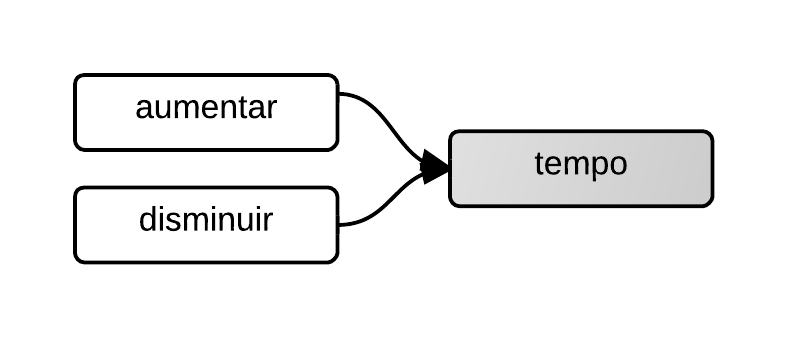
\includegraphics[width=0.6\linewidth]{./graphics/cmd-tempo.png}
\caption{Comandos para aumentar/disminuir el tempo general de al aplicaci\'on}
\label{figure:cmd-tempo-anexo}
\end{minipage}
\end{figure}
 
\subsection{Comandos de Partitura}

Los comandos de las figuras~\ref{figure:cmd-partitura-1-anexo} y~\ref{figure:cmd-partitura-2-anexo} afectan a
la partitura actual, como se explican a continuaci\'on:

\begin{itemize}
    \item \emph{crear nueva  partitura}:  permite crear una nueva partitura en blanco. Utilizaci\'on, ``crear nueva partitura''
    \item \emph{limpiar  partitura}: permite limpiar el contenido de la partitura actual, es decir, borrar todas las notas. Utilizaci\'on, ``limpiar partitura''
    \item \emph{duplicar partitura}: crea una nueva partitura con el mismo contenido que la partitura actual. Utilizaci\'on, ``duplicar partitura''.
\end{itemize}

\begin{figure}[H]
\begin{minipage}[b]{0.5\linewidth}
\centering
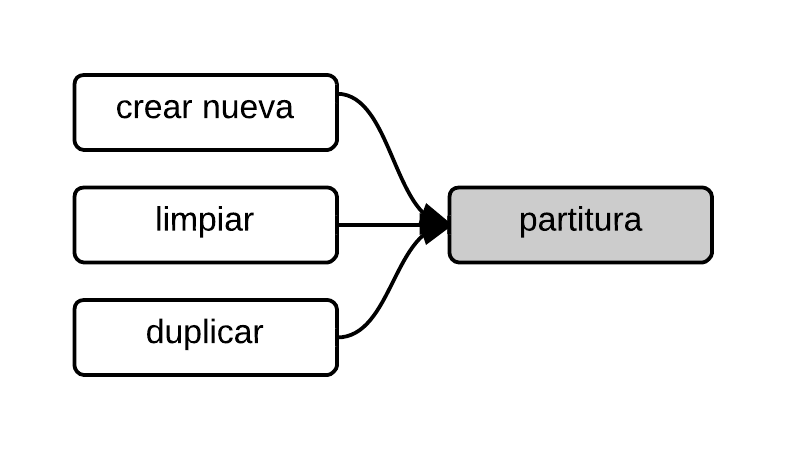
\includegraphics[width=0.6\linewidth]{./graphics/partitura-1.png}
\caption{Comandos para crear, limpiar y duplicar la partitura actual}
\label{figure:cmd-partitura-1-anexo}
\end{minipage}
\quad
\begin{minipage}[b]{0.5\linewidth}
\centering
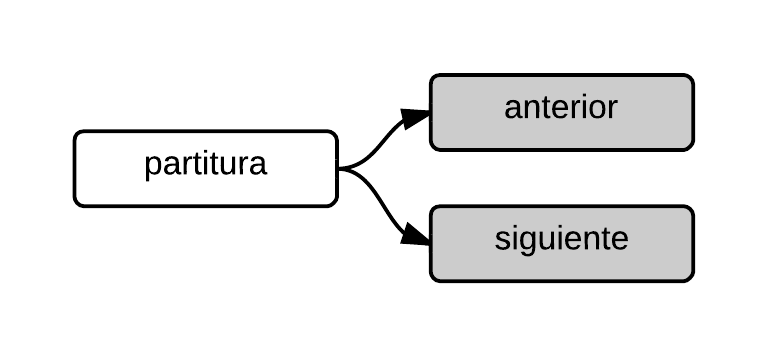
\includegraphics[width=0.6\linewidth]{./graphics/partitura-2.png}
\caption{Comandos para navegar entre partituras}
\label{figure:cmd-partitura-2-anexo}
\end{minipage}
\end{figure} 

Los comandos de la figura~\ref{figure:cmd-partitura-2-anexo} permiten navegar entre partituras.
 
\subsection{Comandos de Pista} 
En la figura~\ref{figure:cmd-pista-1-anexo} puede apreciarse el comando que permite al usuario ubicarse en una pista en particular. Por  
ejemplo, para ubicarse en la pista tres debe decir “pista tres”. Adem\'as de controlar el volumen general de la aplicaci\'on, en 
la figura~\ref{figure:cmd-vol-pista-anexo} se pueden ver los comandos para controlar el volumen de una pista en particular. Para aumentar
el volumen de la pista tres, el usuario debe decir ``aumentar volumen de pista tres''.

\begin{figure}[H]  
\centering
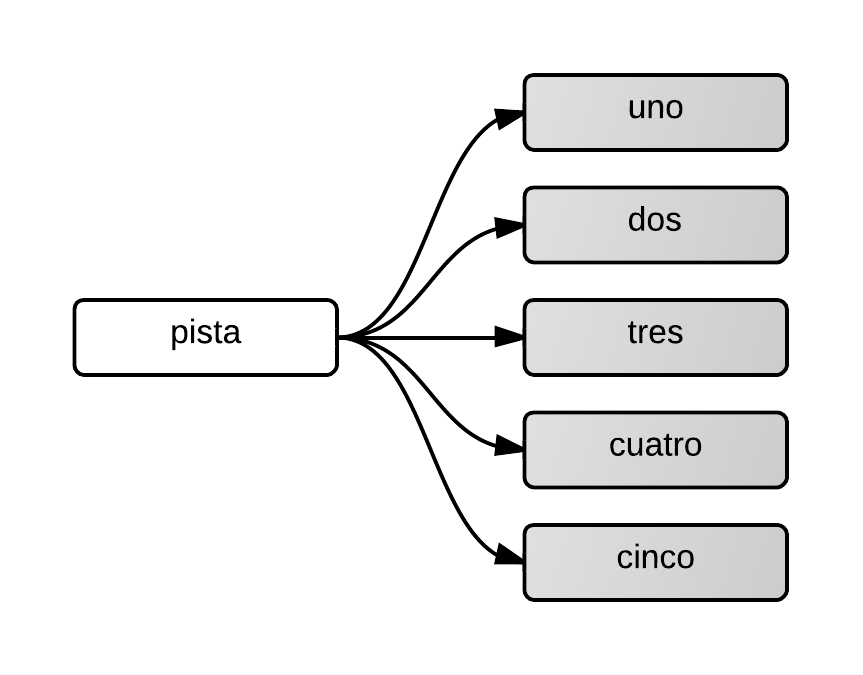
\includegraphics[width=0.6\linewidth]{./graphics/cmd-pista-1.png}
\caption{Comando para ubicarse en una pista}
\label{figure:cmd-pista-1-anexo}
\end{figure}

\begin{figure}[H]  
\begin{minipage}[b]{0.5\linewidth}
\centering
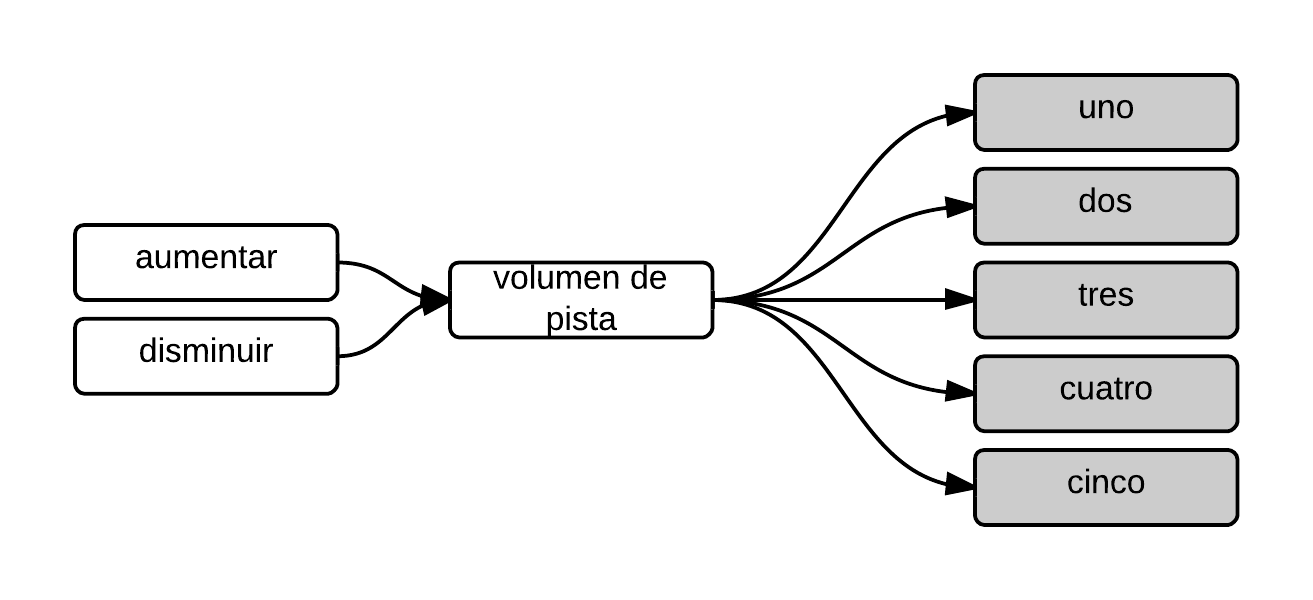
\includegraphics[width=0.8\linewidth]{./graphics/vol-pista.png}
\caption{Comandos para aumentar/disminuir el volumen de una pista en particular}
\label{figure:cmd-vol-pista-anexo}
\end{minipage}
\quad
\begin{minipage}[b]{0.5\linewidth}
\centering
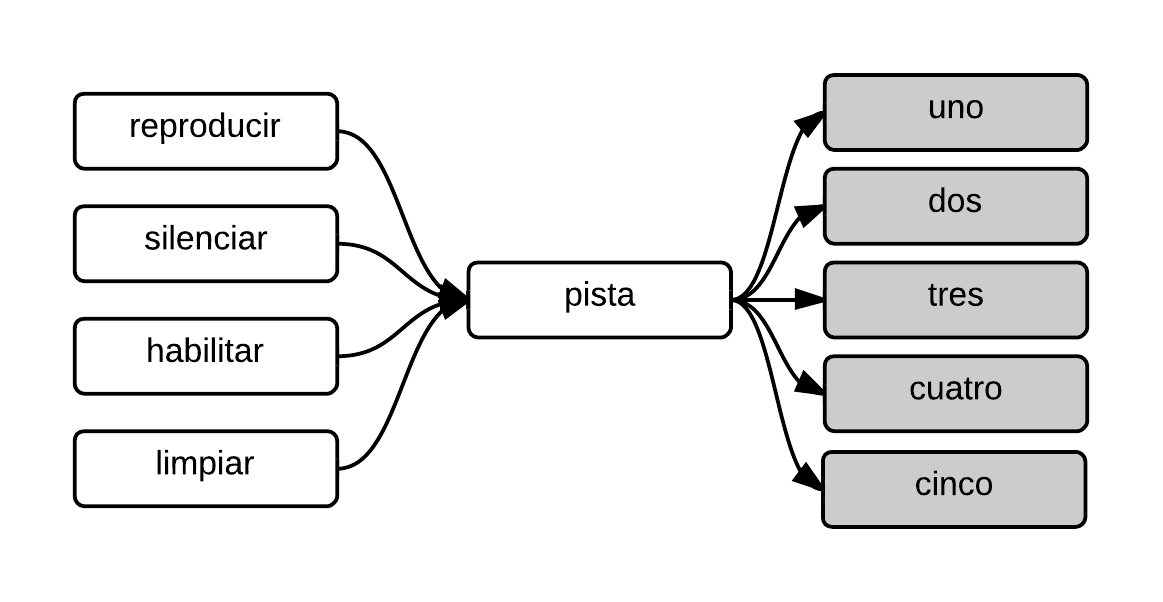
\includegraphics[width=0.9\linewidth]{./graphics/rep-pista.png}
\caption{Comandos para reproducir, silenciar, habilitar y limpiar una pista en particular}
\label{figure:cmd-rep-pista-anexo}
\end{minipage}
\end{figure}

Los comandos de la figura~\ref{figure:cmd-rep-pista-anexo} permiten: reproducir, silenciar, habilitar y limpiar el contenido de una
pista en particular. Por ejemplo, para reproducir las notas de la pista uno, el usuario debe decir ``reproducir pista uno''. 
Para poder generar distintos tipos de sonidos con \emph{TamTam Listens}, los usuarios de pueden asignar
instrumentos a cada una de las pistas de
la aplicaci\'on, \'esto se puede realizar con los comandos de la figura~\ref{figure:cmd-inst-p1-4} y~\ref{figure:cmd-inst-p5}. Para
asignar el piano a la pista dos, basta con decir ``piano en pista dos''.


\begin{figure}[H]
\centering
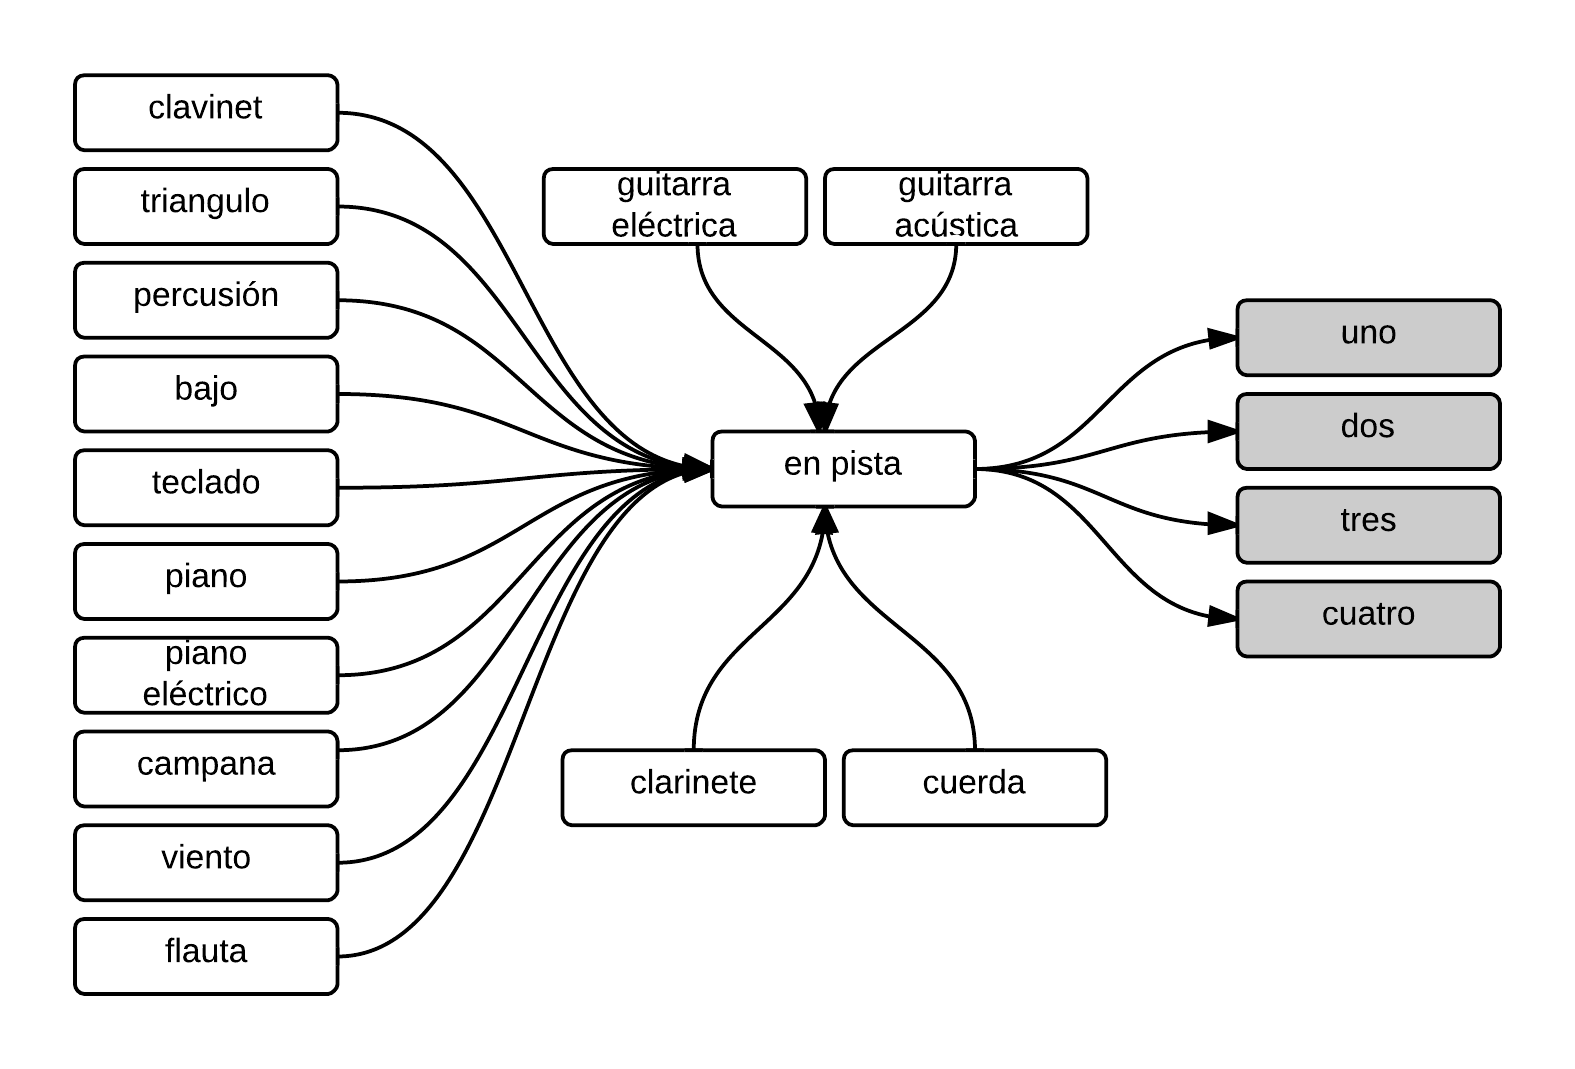
\includegraphics[width=0.8\textwidth]{./graphics/inst-p1-4.png}
\caption{Selecci\'on de instrumento para pistas del uno al cuatro}
\label{figure:cmd-inst-p1-4-anexo}
\end{figure} 

\begin{figure}[H]  
\begin{minipage}[b]{0.5\linewidth}
\centering
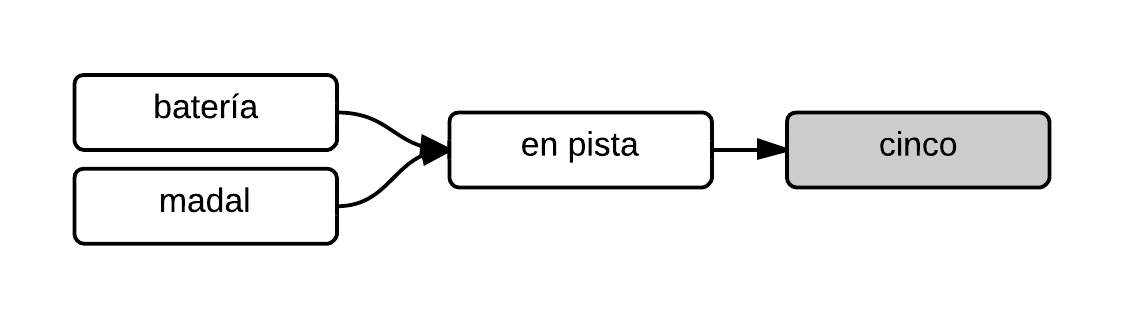
\includegraphics[width=1\linewidth]{./graphics/inst-p5.png}
\caption{Selecci\'on de instrumento para la pista cinco}
\label{figure:cmd-inst-p5-anexo}
\end{minipage}
\quad
\begin{minipage}[b]{0.5\linewidth}
\centering
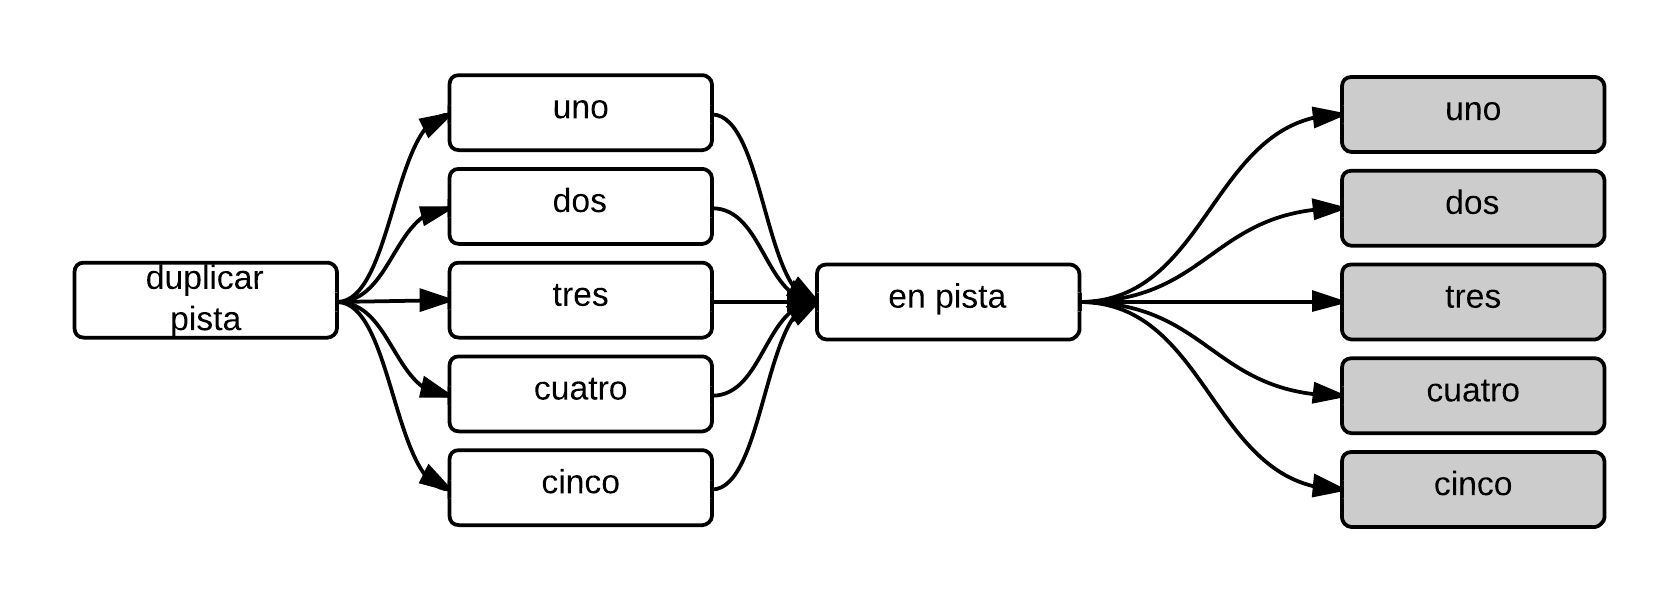
\includegraphics[width=1\linewidth]{./graphics/dup-pista.png}
\caption{Comando para duplicar las notas de una pista en otra}
\label{figure:cmd-dup-pista-anexo}
\end{minipage}
\end{figure}

Generalmente las composiciones tienen cierta secuencia de notas que se repiten para varios instrumentos. El comando de la 
figure~\ref{figure:cmd-dup-pista-anexo} permite duplicar el contenido, es decir las notas, de una pista en otra. Por ejemplo, 
``duplicar pista uno en pista dos'' permite duplicar las notas de la pista uno en la pista dos.

\subsection{Comandos de Comp\'as} 

Estos comandos son muy importantes para la aplicaci\'on ya que permiten crear, modificar, 
eliminar las notas musicales. El comando de la figura~\ref{figure:cmd-compas-anexo} ubica al usuario dentro de una pista en particular. 
Por lo tanto, se debe seleccionar una pista para poder utilizar este comando.

\begin{figure}[H]  
\centering
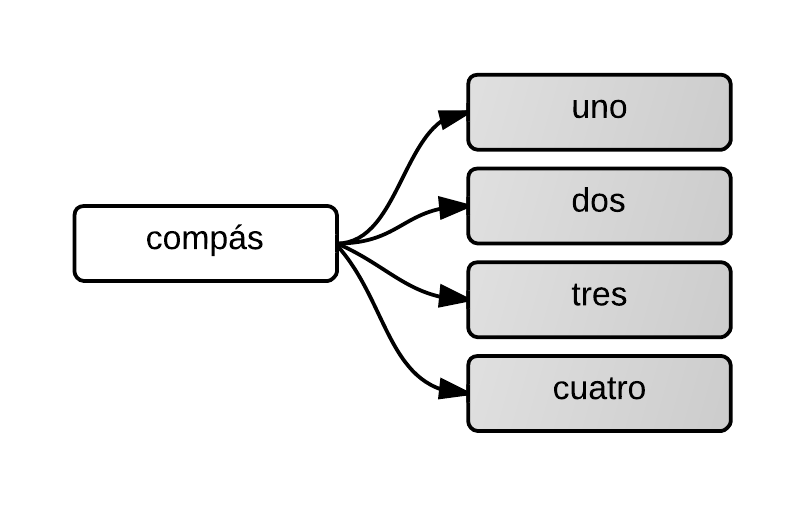
\includegraphics[width=0.4\linewidth]{./graphics/cmd-compas.png}
\caption{Comando para ubicarse en un comp\'as}
\label{figure:cmd-compas-anexo}
\quad
\end{figure}

El comando de la figura~\ref{figure:cmd-crear-nota-anexo} permite crear notas en el  
comp\'as actual, por ejemplo ``crear nota do'' crea la nota do en el comp\'as previamente seleccionado. Por otro lado, en la figura~\ref{figure:cmd-tiempo-compas-anexo} se presenta el comando que permite al usuario ubicarse en un  
tiempo en particular dentro del comp\'as actual. Esto es \'util para crear una nota a partir de ese punto o 
para seleccionar una nota que se encuentre en ese tiempo.

 \begin{figure}[H]
\begin{minipage}[b]{0.5\linewidth}
\centering
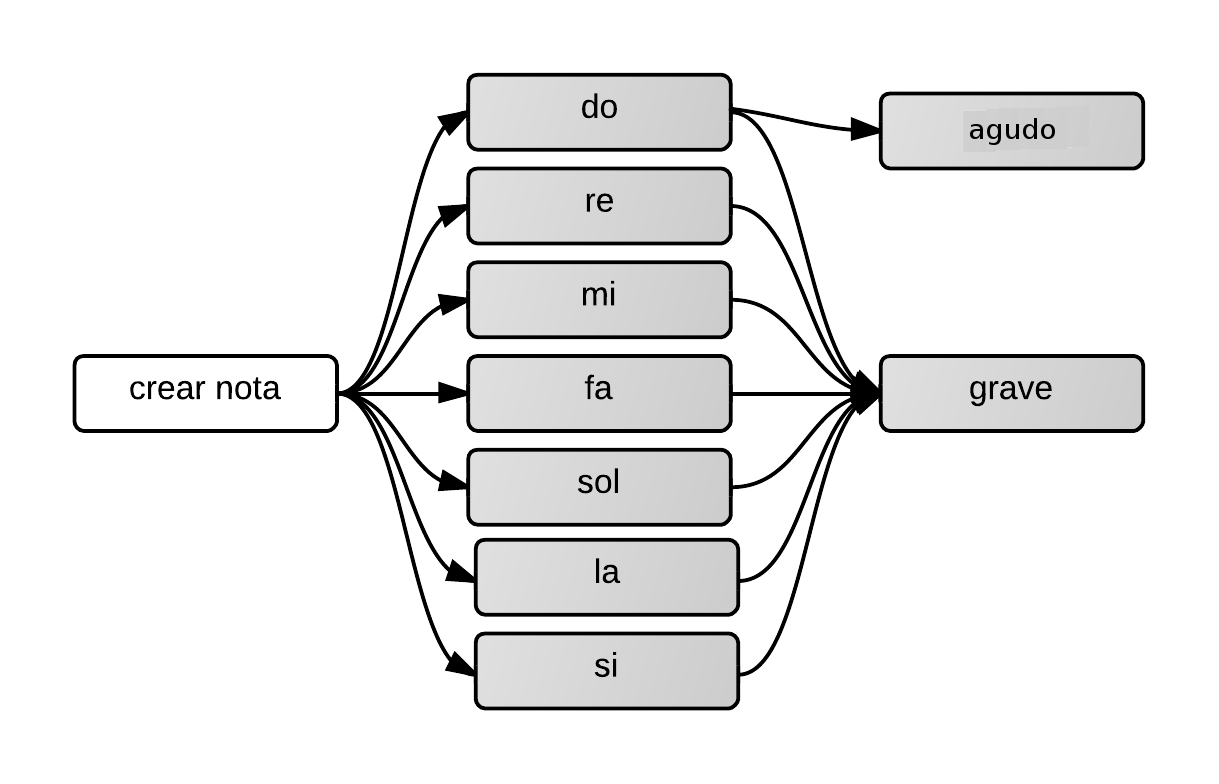
\includegraphics[width=1\linewidth]{./graphics/cmd-crear-nota.png}
\caption{Comando para crear una nota}
\label{figure:cmd-crear-nota-anexo}
\end{minipage}
\quad
\begin{minipage}[b]{0.5\linewidth}
\centering
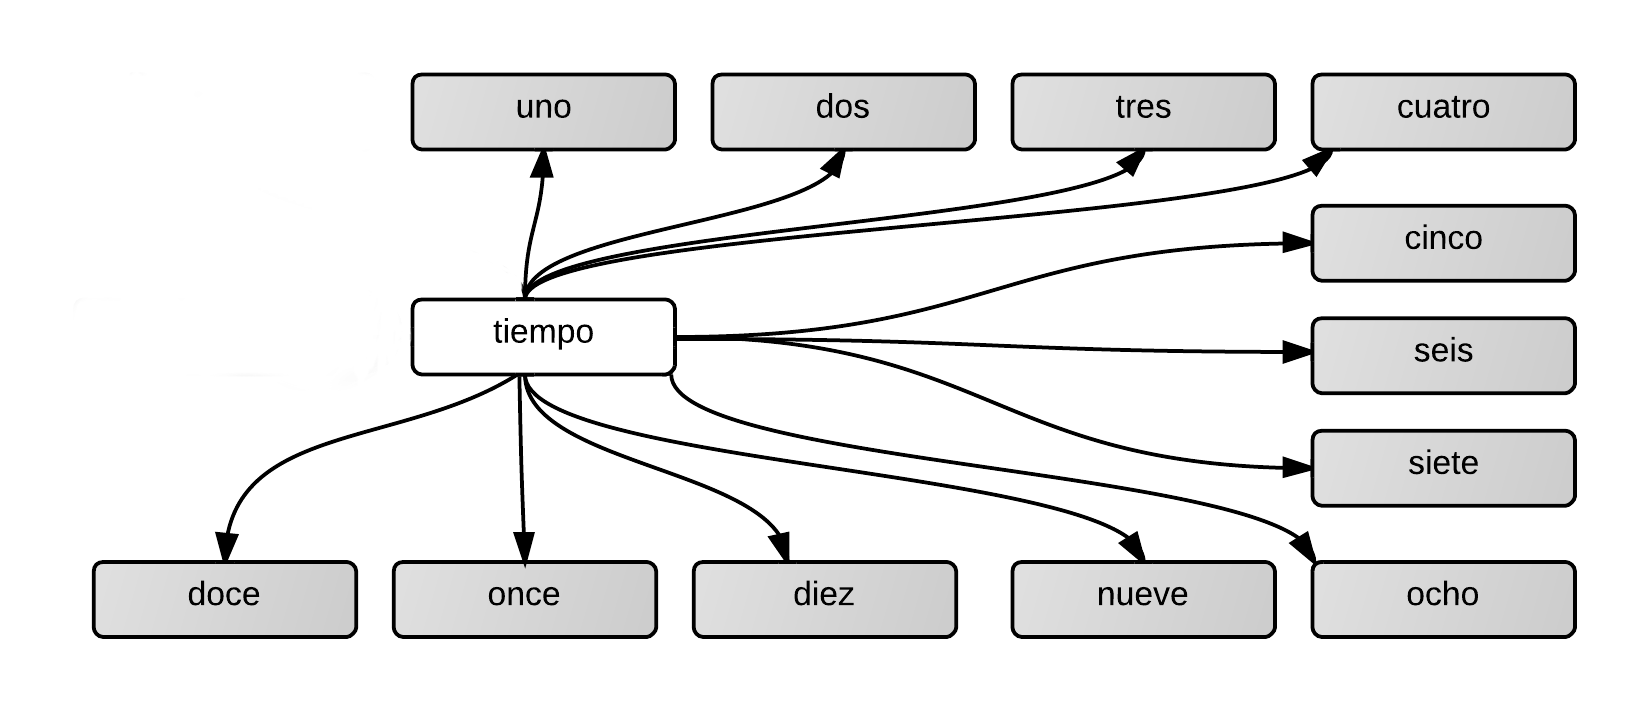
\includegraphics[width=1.1\linewidth]{./graphics/cmd-tiempo-compas.png}
\caption{Comando para ubicarse en un tiempo dado, dentro de un comp\'as}
\label{figure:cmd-tiempo-compas-anexo}
\end{minipage}
\end{figure}

As\'i como puede duplicarse notas de una pista a otra, tambi\'en puede duplicarse una nota de un comp\'as a otro utilizando el comando
de la figura~\ref{figure:cmd-dup-nota-anexo}, por ejemplo ``duplicar en pista uno compas dos'' permite duplicar una nota en el segundo comp\'as de la pista 
uno. Para poder eliminar una nota, previamente seleccionada, el usuario debe utilizar el comando
de la figura~\ref{figure:cmd-del-nota-anexo}.

\begin{figure}[H]
\begin{minipage}[b]{0.5\linewidth}
\centering
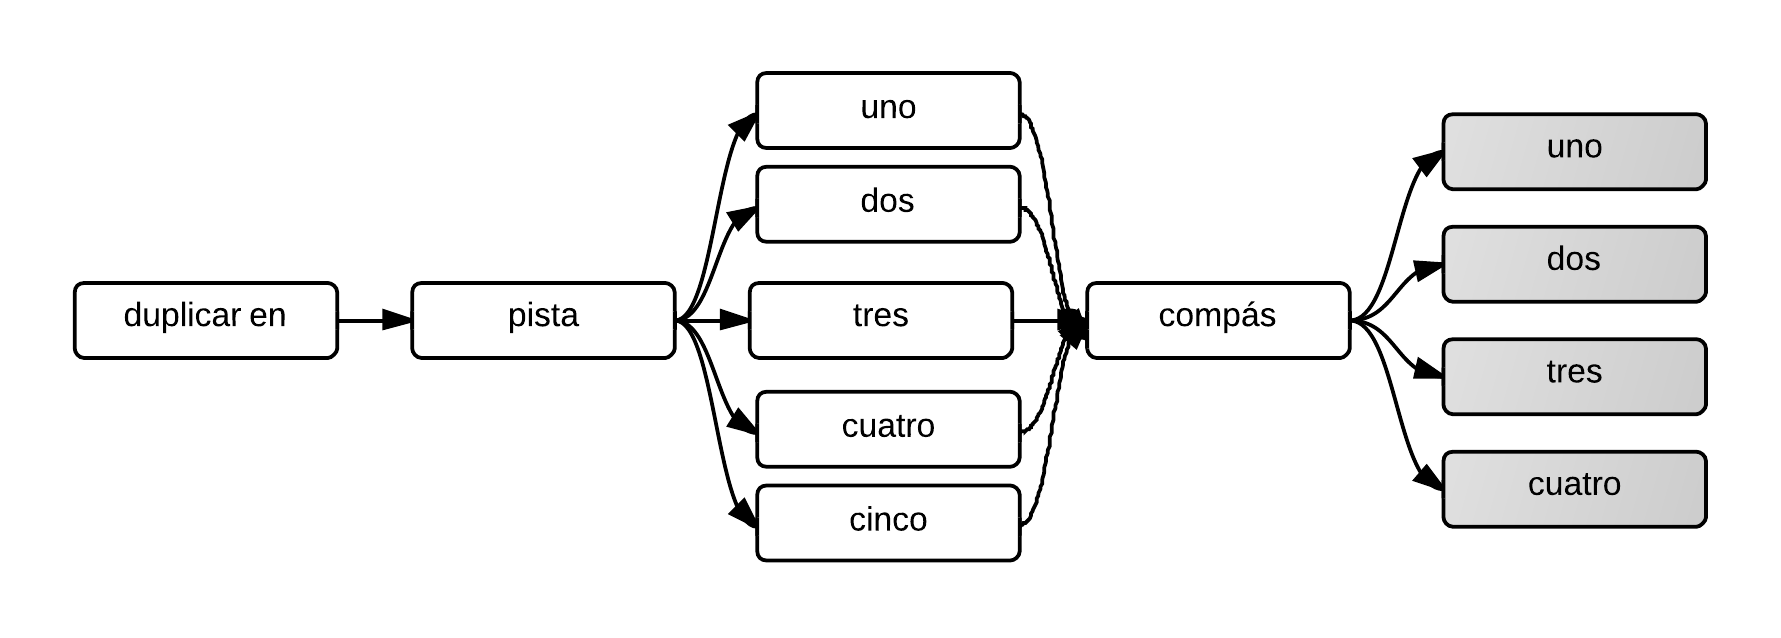
\includegraphics[width=1.2\linewidth]{./graphics/cmd-dup-nota.png}
\caption{Comando para duplicar una nota previamente seleccionada}
\label{figure:cmd-dup-nota-anexo}
\end{minipage}
\quad
\begin{minipage}[b]{0.5\linewidth}
\centering
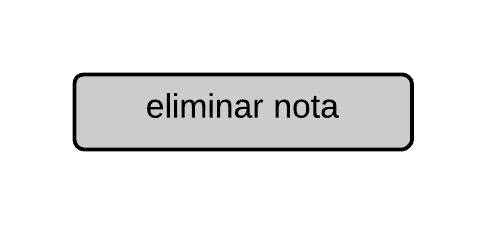
\includegraphics[width=0.5\linewidth]{./graphics/del-note.png}
\caption{Comando para eliminar un nota previamente seleccionada}
\label{figure:cmd-del-nota-anexo}
\end{minipage}
\end{figure}

En la figura~\ref{figure:cmd-dur-anexo} se pude observar el comando que permite modificar la duraci\'on de 
una nota inmediatamente despu\'es de haberla creado o una nota previamente seleccionada. Finalmente, el comando
presentado en la figura~\ref{figure:cmd-note-tiempo-anexo} permite modificar el tiempo en el que inicia la 
nota inmediatamente despu\'es de haberla creado o una nota previamente seleccionada.

\begin{figure}[H]
\begin{minipage}[b]{0.5\linewidth}
\centering
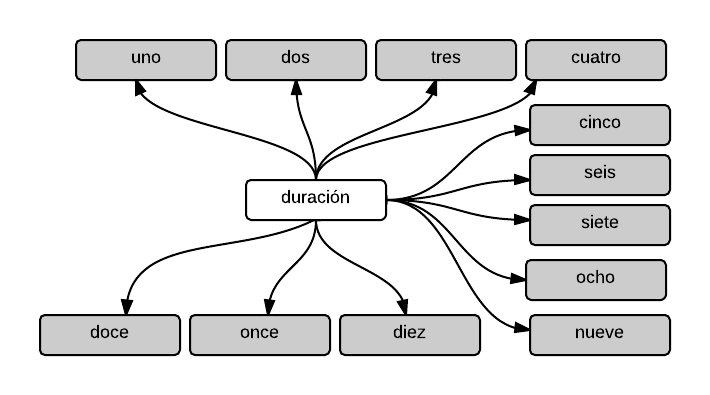
\includegraphics[width=0.9\linewidth]{./graphics/cmd-dur.png}
\caption{Comando que permite configurar la duraci\'on de una nota}
\label{figure:cmd-dur-anexo}
\end{minipage}
\quad
\begin{minipage}[b]{0.5\linewidth}
\centering
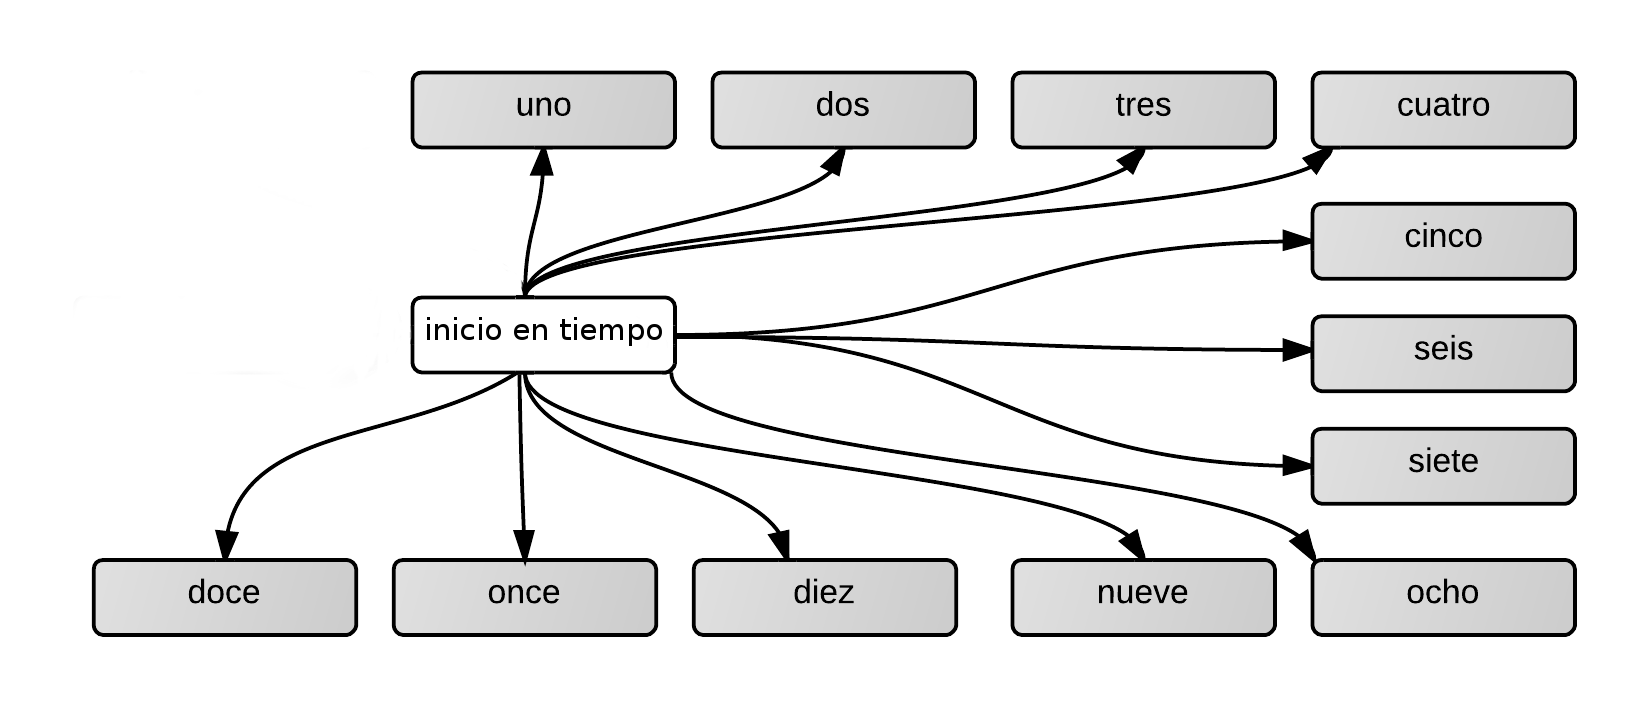
\includegraphics[width=1.1\linewidth]{./graphics/cmd-note-tiempo.png}
\caption{Comando que permite configurar el inicio de una nota dentro del comp\'as}
\label{figure:cmd-note-tiempo-anexo}
\end{minipage}
\end{figure}

\subsection{Diagramas de Interacci\'on}

En esta secci\'on se incluyen algunos diagramas que muestran los pasos necesarios para realizar cierto 
tipo de acciones dentro de la aplicaci\'on.

\subsubsection{Pasos para crear una nota}

En el siguiente diagrama se puede observar los pasos necesarios para crear una nota

\begin{figure}[H]
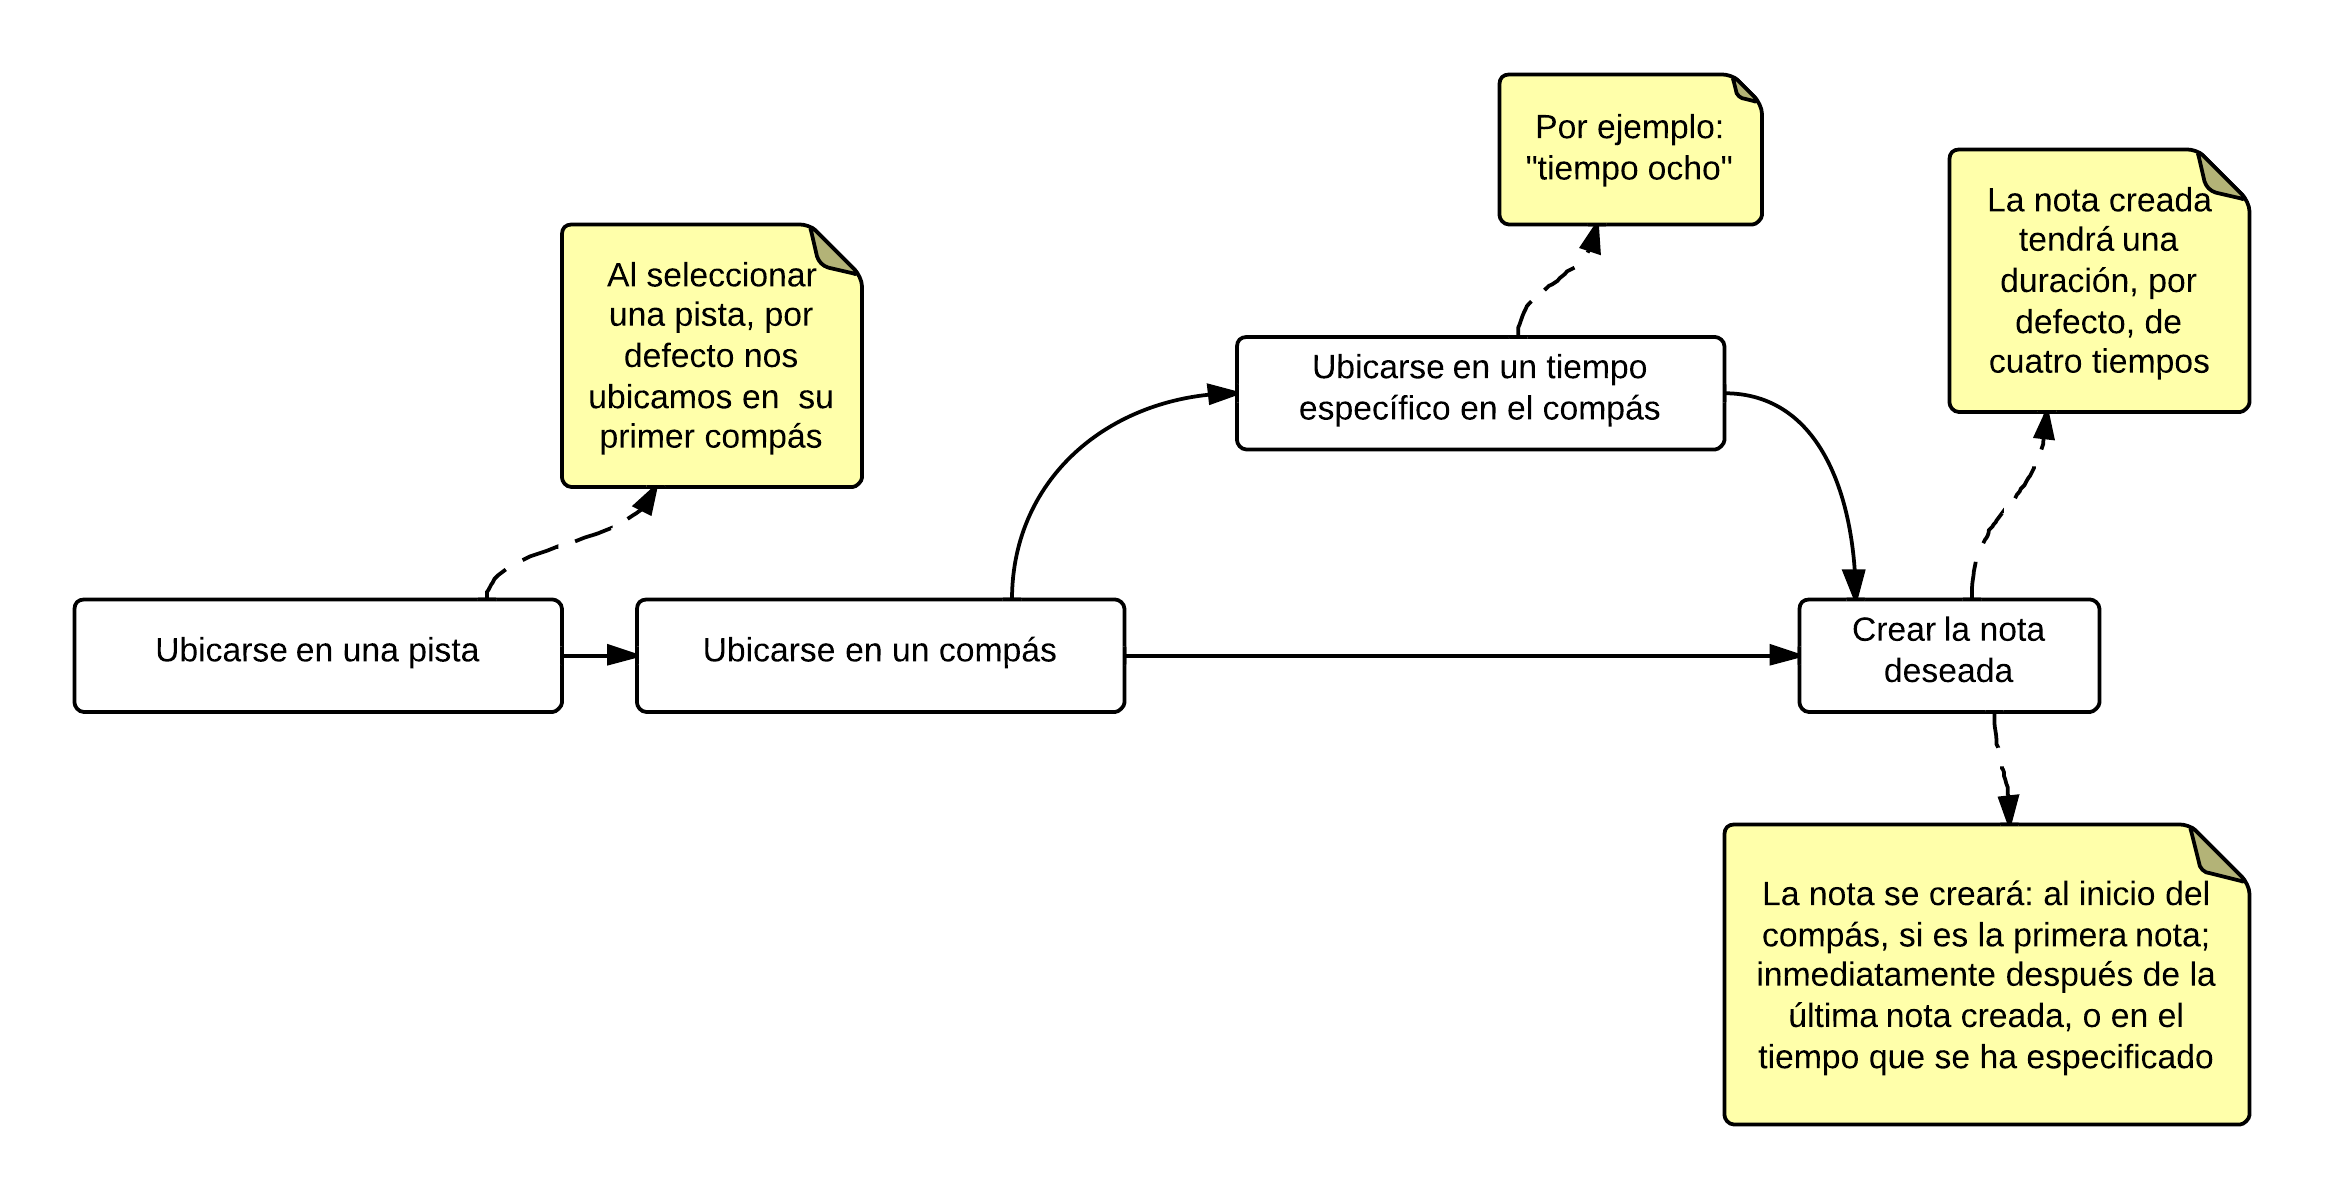
\includegraphics[width=0.9\linewidth]{./graphics/pasos-crear-nota2.png}
\end{figure}
 
\subsubsection{Pasos para modificar una nota reci\'en creada}
Una nota reci\'en creada puede autom\'aticamente ser modificada alterando su duraci\'on y/o 
tiempo de inicio en el comp\'as, como se puede ver en el siguiente diagrama.

\begin{figure}[H]
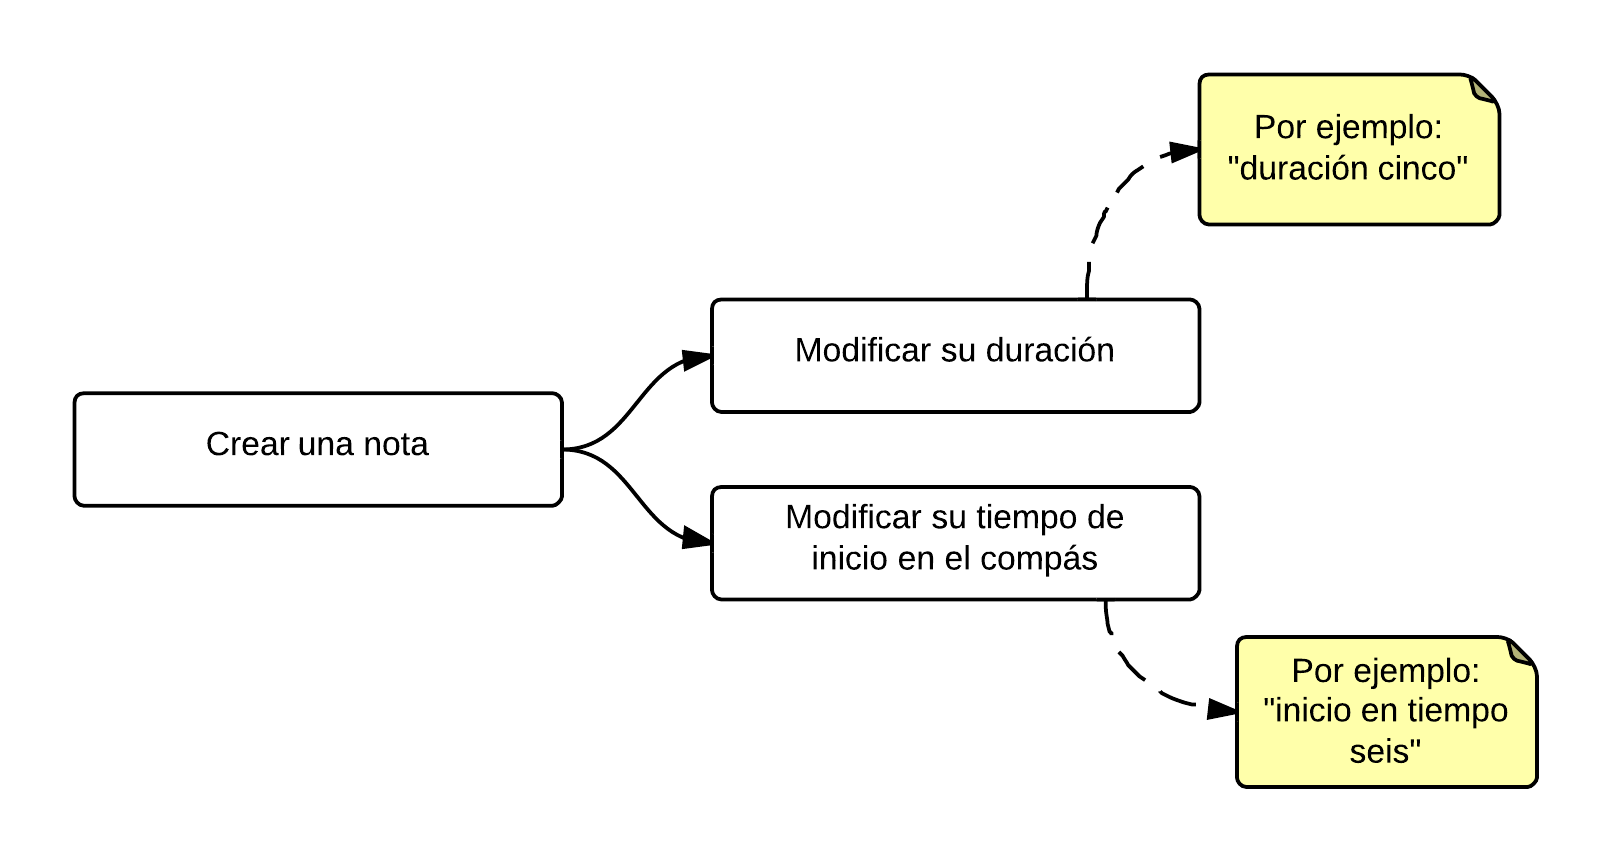
\includegraphics[width=0.9\linewidth]{./graphics/pasos-modificar-nota-recien-creada.png}
\end{figure}
 
\subsubsection{Pasos para modificar una nota}
Para poder modificar una nota en particular (no necesariamente una que acabamos de crear) debemos 
primero seleccionar la nota, para luego seguir de manera similar al diagrama anterior.

\begin{figure}[H]
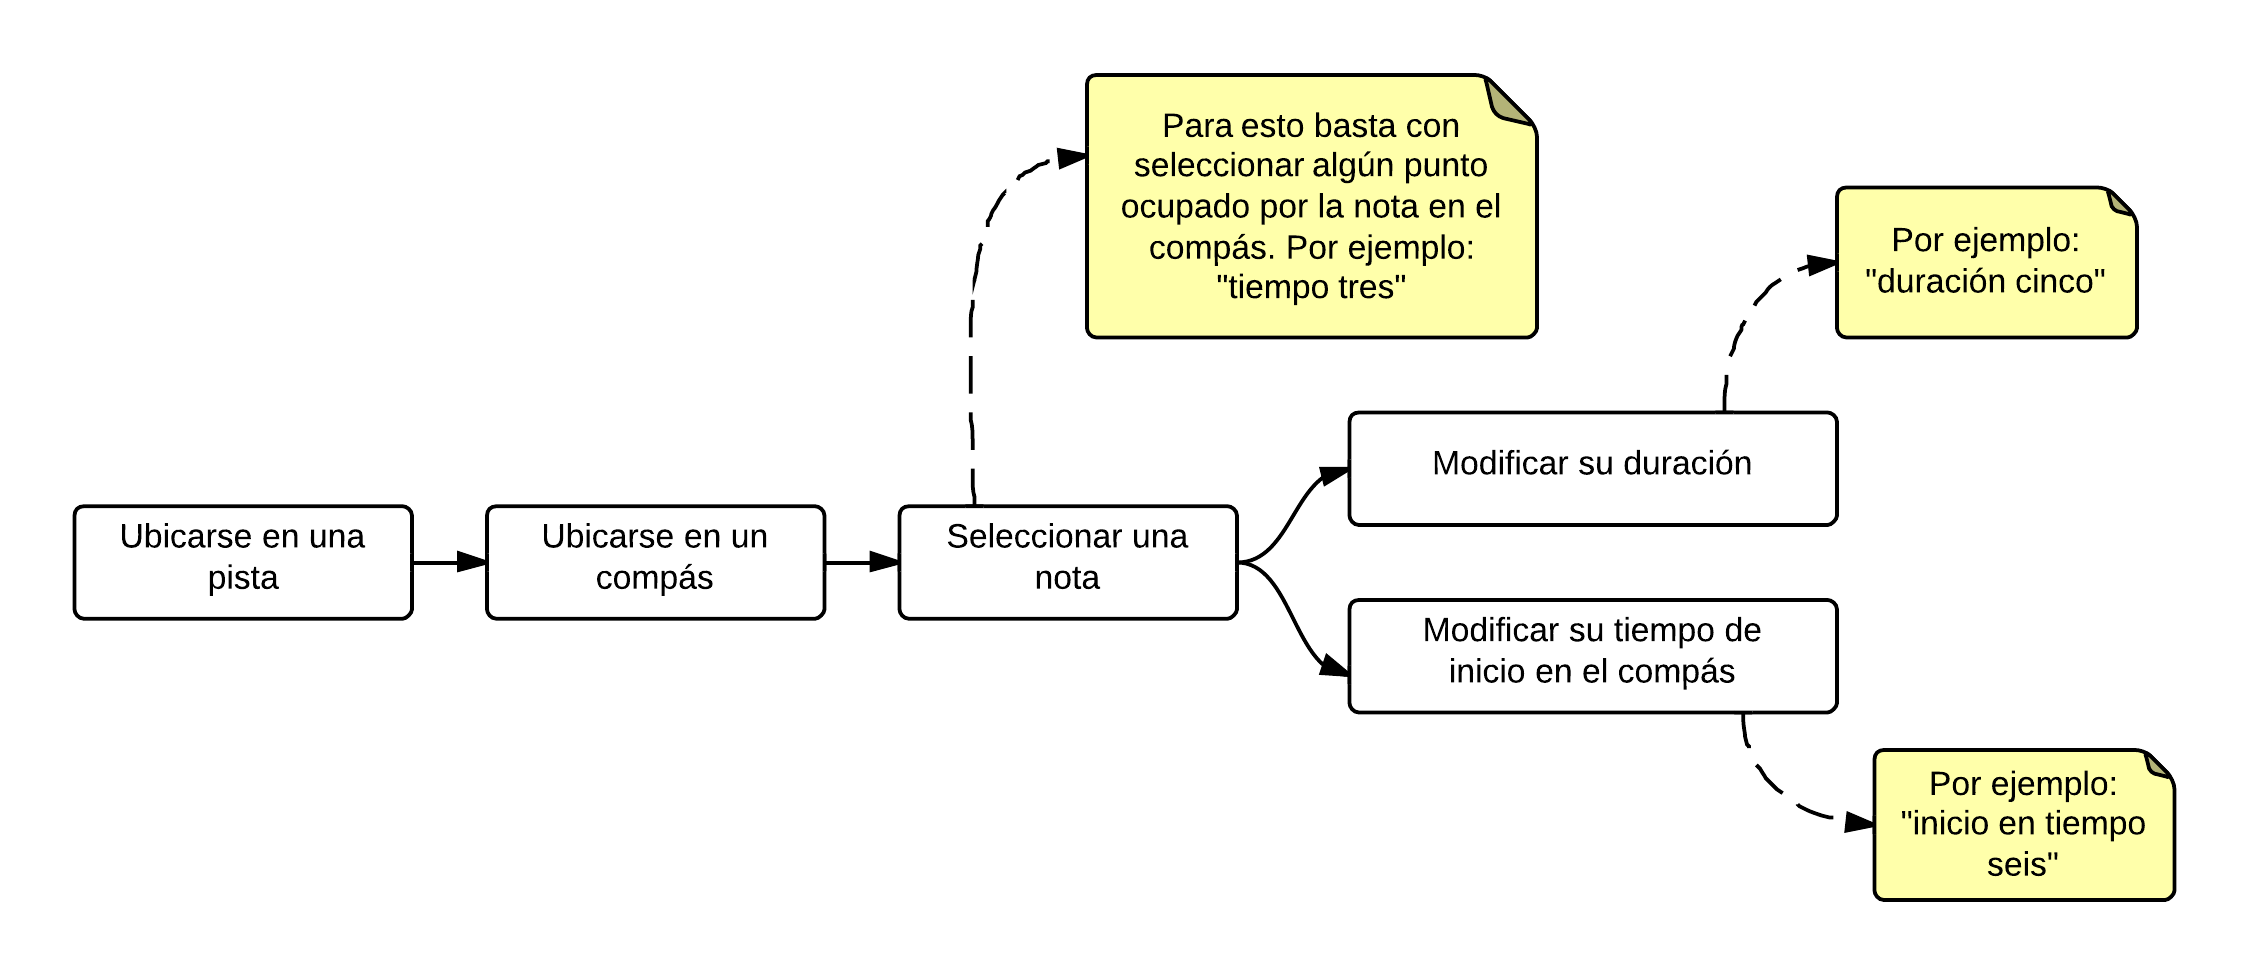
\includegraphics[width=0.9\linewidth]{./graphics/pasos-modificar-nota-seleccionar.png}
\end{figure}

\subsection{Tutoriales de Uso}
En esta secci\'on se incluyen explicaciones breves de algunos ejemplos de uso de la aplicaci\'on, de modo a facilitar el proceso de aprendizaje.

\subsubsection{Componiendo una escala simple}

\begin{enumerate}
\item Para empezar, debemos obtener una partitura en blanco. Lo conseguimos pronunciando el comando: ``Crear Nueva M\'usica''.
\item Seleccionamos los instrumentos que queremos utilizar, diciendo:
\begin{itemize}
    \item ``Piano en Pista Uno''
    \item ``Guitarra El\'ectrica en Pista Dos''
    \item ``Teclado en Pista Tres''
    \item ``Flauta en Pista Cuatro''
\end{itemize}
\item Antes de crear las notas, debemos ubicarnos en el punto donde queremos empezar:
\begin{itemize}
\item ``Pista Uno'' : el comando nos ubica en el tiempo uno, del comp\'as uno de la pista uno.
\end{itemize}
    Si quisi\'esemos empezar en el tiempo uno del comp\'as dos, bastar\'ia con decir:
\begin{itemize}
\item ``Comp\'as Dos''
\end{itemize}
    En caso de querer empezar en el tiempo siete, decimos:
\begin{itemize}
\item ``Tiempo Siete''
\end{itemize}
\item Ya seleccionado el punto inicial, estamos listos para crear las notas :
\begin{itemize}
    \item ``Crear Nota Do''
    \item ``Crear Nota Re''
    \item ``Crear Nota Mi''
    \item ``Crear Nota Fa''
    \item ``Crear Nota Sol''
    \item ``Crear Nota La''
    \item ``Crear Nota Si''
\end{itemize}
\item Como no queremos trabajar de m\'as, duplicamos las pistas para escuchar los dem\'as instrumentos.
\begin{itemize}
    \item ``Duplicar Pista Uno en Pista Dos''
    \item  ``Duplicar Pista Dos en Pista Tres''
    \item ``Duplicar Pista Tres en Pista Cuatro''
\end{itemize}
\item As\'i de f\'acil. Para escuchar nuestra m\'usica: ``Reproducir M\'usica''.
\end{enumerate}
 
\subsubsection{Modificando una Nota}

Si queremos cambiar una nota luego de su creaci\'on, estos son los pasos a seguir:

\begin{enumerate}
\item Primero, debemos seleccionar la nota. Si la acabamos de crear, la nota se 
    encuentra seleccionada, por lo que este paso puede omitirse.
    En caso contrario, basta con seleccionar alg\'un punto ocupado por la nota en la partitura.
    Por ejemplo, para seleccionar una nota en el comienzo del segundo comp\'as de la pista tres,  dir\'iamos:
    \begin{itemize}
        \item ``Pista Tres''
        \item ``Comp\'as Dos''
        \item ``Tiempo Uno''
     \end{itemize}
\item Una vez seleccionada la nota, podemos cambiar su duraci\'on (por defecto 4 tiempos) a 9 tiempos, podemos decir: 
     ``Duraci\'on Nueve''.
\item Si queremos desplazar el inicio de la nota al quinto tiempo, decimos ``Inicio en Tiempo Cinco''.
\item Supongamos que la nota existente es un Fa y queremos cambiarla por un Sol. Para reemplazar la 
     nota por otra, basta con crear la nueva nota en su lugar diciendo ``Crear Nota Sol''.
\item Si nada nos convence, y preferimos eliminar la nota seleccionada, decimos ``Eliminar Nota''.
\end{enumerate}
